\documentclass[a4paper,14pt]{article}
\usepackage{float}
\usepackage{extsizes}
\usepackage{amsmath}
\usepackage{amssymb}
\everymath{\displaystyle}
\usepackage{geometry}
\usepackage{fancyhdr}
\usepackage{multicol}
\usepackage{graphicx}
\usepackage[brazil]{babel}
\usepackage[shortlabels]{enumitem}
\usepackage{cancel}
\usepackage{textcomp}
\columnsep=2cm
\hoffset=0cm
\textwidth=8cm
\setlength{\columnseprule}{.1pt}
\setlength{\columnsep}{2cm}
\renewcommand{\headrulewidth}{0pt}
\geometry{top=1in, bottom=1in, left=0.7in, right=0.5in}

\pagestyle{fancy}
\fancyhf{}
\fancyfoot[C]{\thepage}

\begin{document}
	
	\noindent\textbf{Matemática} 
	
	\begin{center}Operações com números inteiros, expressões numéricas e problemas \\ (Versão professor)
	\end{center}
	
	\noindent\textbf{Nome:} \underline{\hspace{10cm}}
	\noindent\textbf{Data:} \underline{\hspace{4cm}}
	
	%\section*{Questões de Matemática}
	
	
    \begin{multicols}{2}
		\begin{enumerate}
			\item Carlos realizou o controle financeiro mensal da sua loja de esfiha pelo período de seis meses e o registrou em um gráfico.
			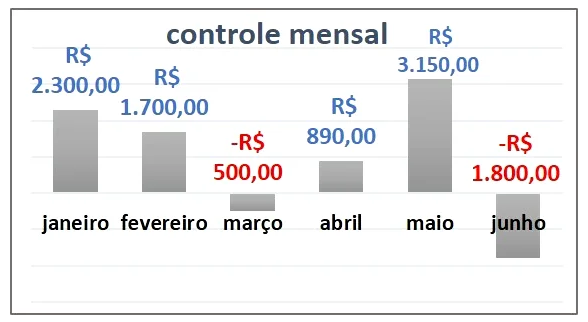
\includegraphics[width=1\linewidth]{Leonardo_imagens/imagem1}
			a) Segundo o gráfico, qual o resultado do primeiro trimestre?\\\\\\\\\\
			
			b) Qual a diferença entre o melhor e o pior resultado do semestre?\\\\\\\\\\
			
			c) Qual foi o saldo semestral?\\\\\\\\\\\\\\
			
			\fontfamily{phv} \selectfont
			
			Resposta:
			
			a) 1º trimestre (janeiro + fevereiro + março) \\\\
			2300 + 1700 +(-500) = \\
			4000 - 500 = \\
			3500 \\
			
			O resultado do primeiro trimestre foi de R\$ 3 500,00.
			
			b) O melhor mês foi maio com R\$ 3 150,00 de lucro e o pior foi junho com R\$ 1 800,00 de prejuízo. \\
			
			\fontsize{10}{\baselineskip} \selectfont
			
			3 150 + (-1 800) = 3 150 – 1 800 = 1 350 \\
			
			\fontsize{12}{\baselineskip} \selectfont
			
			A diferença foi de R\$ 1 350,00 entre o melhor e pior resultado mensal.\\
			
			c) É a soma dos totais de cada mês. \\
			\fontsize{10}{\baselineskip} \selectfont
			
			2300 + 1700 +(-500) + 890 + 3150 +(-1800) = \\
			4000 - 500 + 890 + 3150 - 1800 = \\
			3500 + 890 + 3150 - 1800 = \\
			4390 + 3150 - 1800 = \\
			7540 - 1800 = \\
			5740 \\\\
			
			\fontsize{14}{\baselineskip} \selectfont
			
			O resultado semestral foi de R\$ 5 740,00.
			
			\fontfamily{cmr} \selectfont
			
			\item Situação Problema \\\\
			Patrícia é proprietária de uma loja de rações para cães e gatos. Este mês ela adquiriu 400 kg de ração para cachorros a um custo de R\$ 12,00 o quilograma e, 100 kg de ração para gatos ao custo de R\$ 7,50 o quilograma. Considerando que o preço de venda da ração para cachorro é de R\$ 22,00 e para gatos R\$ 19,50 e que até o momento ela vendeu 143 kg de ração de cachorro e 86 kg de ração para gatos, em relação ao investimento inicial, ela já obteve lucro ou ainda não cobriu o custo? \\
			
			Represente a situação com operações e represente utilizando números inteiros. \\
			
			\fontfamily{phv} \selectfont
			Resposta:\\
			
			Cálculo do investimento inicial ou custo.\\
			400 $\cdot$ 12 = 4 800\\
			100 $\cdot$ 7,50 = 750\\
			\\
			4 800 + 750 = 5 550\\
			\\
			O custo foi de R\$ 5 550.\\
			\\
			Valor arrecadado com as vendas até o momento.\\\\
			22 $\cdot$ 143 = 3 146\\
			19,50 $\cdot$ 86 = 1 677\\
			\\
			3 146 + 1 677 = 4 823\\
			\\
			O total arrecadado foi de R\$ 4 823,00.\\
			\\
			Fazendo a diferença 4 823 - 5 550 = -727.\\
			
			Até o momento faltam R\$ 727,00 para Patrícia cobrir o custo inicial.
			
			\fontfamily{cmr} \selectfont
			
			\item Efetue as operações com números inteiros:
			\begin{enumerate}[a)]
				\item $-123 + 235 + 899 = $ \\
				
				Resposta: \\
				
				$-123 + 235 + 899 = $ \\
				$-123 + 1134 = $ \\
				$1011$ \\
				
				\item $(-21)-(+81)-(-50) = $ \\
				
				Resposta: \\
				
				$(-21)-(+81)-(-50)$ \\
				$-21 - 81 + 50$ \\
				$-102 + 50$ \\
				$-52$ \\\\\\\\\\\\\\\\
				
				\item $(-19)(+30)(-2) = $ \\
				
				Resposta: \\
				
				$(-19)(+30)(-2)$ \\
				$-19 \times 30 \times -2$ \\
				$-570 \times -2$ \\
				$1140$ \\
				
				\item $(+90):(-30) = $ \\
				
				Resposta: \\ 
				
				$(+90):(-30)$ \\
				$90 \div -30$ \\
				$-3$ \\
				
				\item $(3^2 + 6^3) = $
				
				Resposta: \\
				
				$(3^2 + 6^3)$ \\ 
				$(3^2) + (6^3)$ \\
				$(3 \times 3) + (6 \times 6 \times 6)$ \\
				$9 + 216$ \\
				$225$ \\
				
				\item $5(10^2 + 11^2) = $ \\
				
				Resposta: \\
				
				$5(10^2 + 11^2)$ \\
				$5(100 + 121)$ \\
				$5(221)$ \\
				$1105$ \\\\\\\\\\\\
				
				\item $(20 + 10 -((15):(+5))) = $
				
				Resposta: \\
				
				$(20 + 10 -((15):(5)))$ \\
				$(20 + 10 -(3))$ \\
				$(30 - 3)$ \\
				$27$ \\\\\\
				
				\item $(-5)(+3)-(9)^5 = $ \\
				
				Resposta: \\ 
				
				$-15 - 59049$ \\
				$-59064$ \\
				
				\item $(-1)^{100} \cdot (-1)^{101} -(1)^0 = $ \\
				
				Resposta: \\
				
				$1 \cdot (-1) - 1$ \\
				$-1 - 1$ \\
				$-2$ \\
				
				\item $(90)^0 + 155 + 1590^0 - 3 = $ \\
				
				Resposta: \\
				
				$1 + 155 + 1 - 3$ \\
				$154$ \\
			\end{enumerate}
        \end{enumerate}
    $~$ \\ $~$ \\ $~$ \\ $~$ \\ $~$ \\ $~$ \\ $~$
    \end{multicols}
\end{document}